\section{Scenario and Problem}
Yellow-Spaceship \cite{Yellow-Spaceship} is a space shooter game implemented using Pygame \cite{PyGame} in which the
player, a battleship, fights a number of enemies by shooting at them while dodging their fire:
enemies can be aliens or spaceships. The player and the enemies move horizontally and
can fire: actions can be defined as “move left”, “move right”, “do not move”, “fire”; moving
and firing can be performed simultaneously, so in the end, we have in total 6 possible
combinations of actions. Levels are structured such that there are always 2 aliens in
each level except for levels multiple of 5 where, instead, there is an enemy spaceship. The battleship
and the enemy spaceship have an initial health of 50 life points whereas the health of enemy
aliens increases as the level increases. Initially, the alien health is set to 10 life points and
gradually increases by 8 life points every 10 levels. The laser damage for the spaceship is
fixed to 1 life point whereas the one of enemies is initially set to 2 life points and gradually
increases by 6 life points every 10 levels. As the game proceeds, it becomes more difficult
to beat the enemies, enemy lasers become more lethal and each level takes longer to be completed. 
Fig. \ref{fig:game_screenshot} shows a screenshot of the game.

\begin{figure}[ht]
\centerline{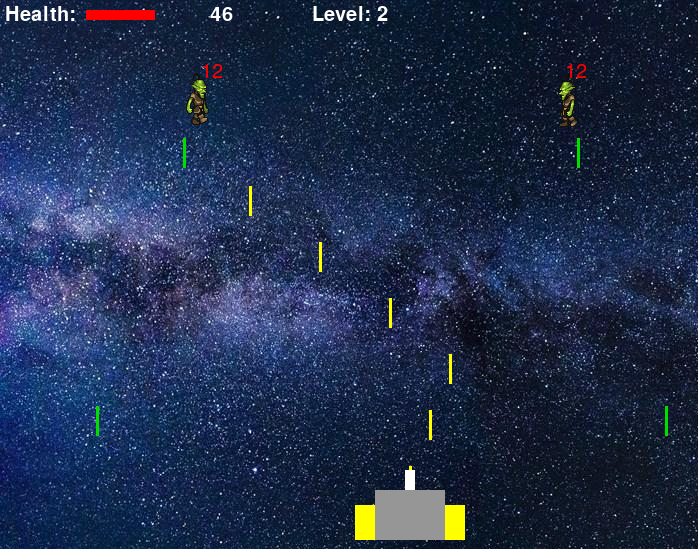
\includegraphics[scale=0.35]{screenshot.png}}
\caption{Screenshot of the Yellow-Spaceship game \cite{Yellow-Spaceship}.}
\label{fig:game_screenshot}
\end{figure}

The number of levels is not bound and the aim of the game is to kill as many enemies as
possible and reach the highest level without losing the whole life.
